%pb
\documentclass[../../main/main.tex]{subfiles}

\begin{document}


%%%%%%%%%%%%%%%%%%%%% Chapter Patrol Base Operations %%%%%%%%%%%%%%%
\chapter{Patrol Base Operations}\label{chp:pb}
   %%%%%%%%%%%%%%%%%%%% Section Motivation %%%%%%%%%%%%%%%%%%%%%%
The patrol base operations are modeled as a modularized hierarchy of secure state machines.  This model is a collaborative effort between the author of this thesis and a subject matter expert Jesse Nathaniel Hall from the U.S. Army.  But, the details with regards to translating the Ranger Handbook into the model is primarily the work of Jesse Hall.  He deserves a lot of credit for his work on this project.  

To demonstrate properties of complete mediation on the patrol base operations, they are modeled as a hierarchy of secure state machines (SSMs). The hierarchy and modularization manage the complexity of the operations.  The \glspl{ssm} constrain the behavior of the operations such that authentication and authorization can be formally verified and documented with an access-control logic and computer-aided reasoning.

This chapter describes the structure and details of the model.  Chapter  \ref{sec:ssm} describes SSMs in more detail.

   %%%%%%%%%%%%%%%%%%% Section Ranger Handbook Description %%%%%%%%%%%%%
\section{Patrol Base Operations}
Patrol base operations are described in the United States Army Ranger Handbook \cite{rangermanual} in chapter 7 (2017 edition).  The mission activity specification for the patrol base operations are shown in table \ref{pbtab}

\parskip=8pt
\begin{table}[h!]
\begin{center}
\begin{tabular}{ | m{3.3em} | m{3.8cm}| m{9cm} | } 
\hline
\multicolumn{3}{|c|}{Patrol Base Operations: Mission Activity Specification} \\
\hline \hline
Purpose & A system to & establish a security perimeter when a squad or platoon halts for an extended period of time \\ 
\hline
Method & by means of  & planning, reconnaissance, security, control, and common sense  \\ 
\hline
Goal & in order to & 
\begin{itemize}
\item avoid detection
\item hide a unit during a long, detailed reconnaissance
\item perform maintenance on weapons, equipment, eat, and rest
\item plan and issue orders
\item reorganize after infiltrating an enemy area
\item establish a base from which to execute several consecutive or concurrent operations
\end{itemize}

 \\ 
\hline
\end{tabular}
\end{center}
\caption{Mission Activity Specification for Patrol Base Operations.  Adapted from the U.S. Army Ranger Handbook 2017 \cite{rangermanual}.}
\label{pbtab}
\end{table}
\parskip=18pt

%   %%%%%%%%%%%%%%%%%%% Section Describing The Patrol Base Operations %%%%%%%%
%\section{Modeling the Patrol Base Operations from the Ranger Handbook}\label{sec:modelingpb}
%\glsresetall[\acronymtype]
%

\section{Overview of The Model}\label{sec:overview}

Each level of the hierarchy of \gls{ssm}s represents a level of abstraction of the patrol base operations. The most abstract level of the hierarchy is the top level \gls{ssm}.  A diagram of this most abstract level is shown in figure \ref{pbtoplevel}.

\begin{figure}[h]
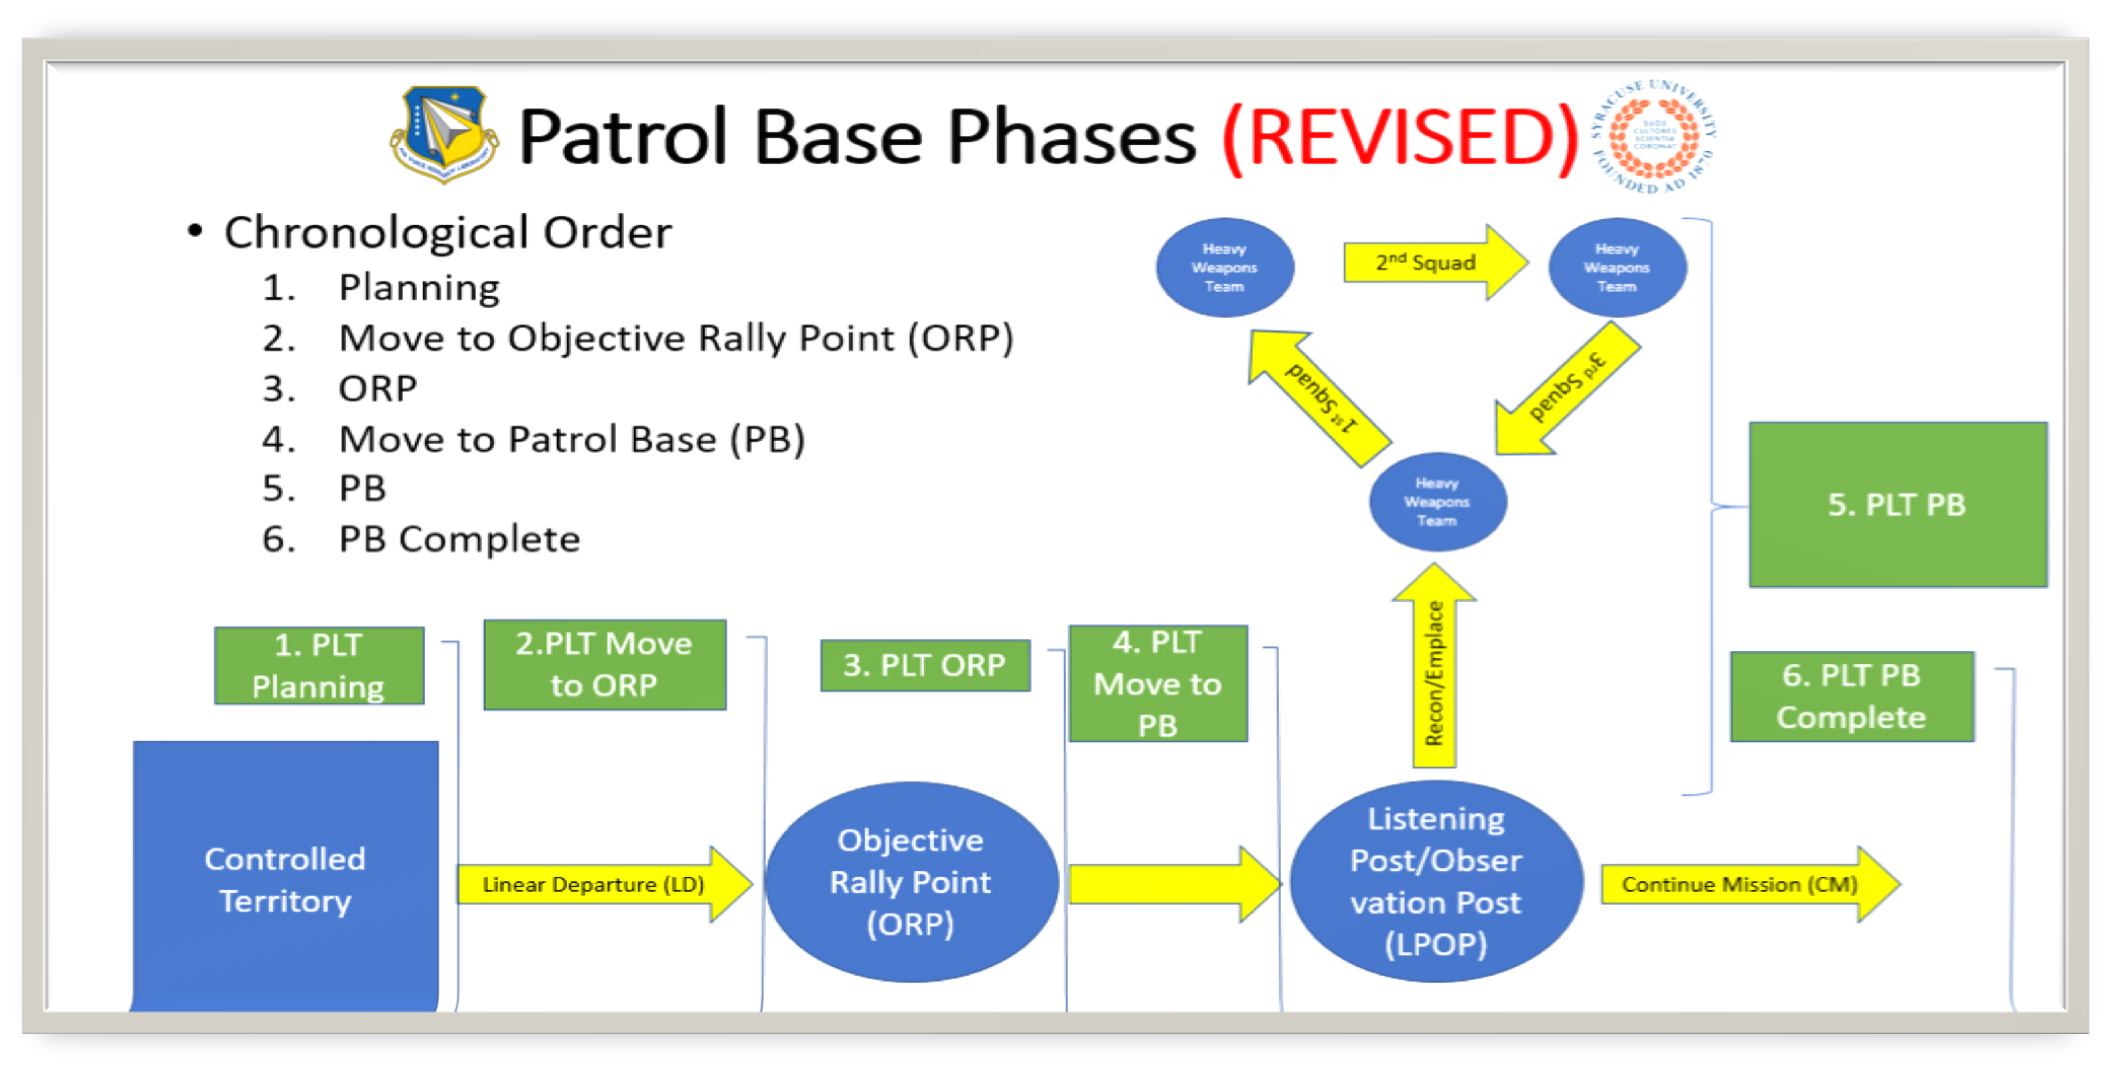
\includegraphics[width=\textwidth]{../figures/pbtoplevel}
\caption{\label{pbtoplevel}A diagram of the most abstract level in the hierarchy of secure state machines.  Image generated by Jesse Nathaniel Hall.}
\end{figure}

The diagram describes a chronological order of abstract phases (modeled as states) of the patrol base operations.  (1) The operations begin with the planning phase. (2)  Next, they move to the \gls{orp}. (3) At the \gls{orp}, operations commence. (4)  When these are complete, the patrol base operations move to the actual patrol base.  (5)  At the patrol base, operations proceed.  (6)  Finally, the patrol base operations are complete.  The last phase is an end phase (actual withdraw, etc. of the operations are included in the 5th phase).


The next level of abstraction in the hierarchy of \gls{ssm} represents a horizontal slice through the patrol base operations. This slice describes the patrol base operations at a lower level of abstraction.  It expands each of the states in the top level (except for the last state PB Complete).  For example, the planning phase (1) in figure \ref{pbtoplevel} is expanded into an \gls{ssm} of its own.  This is called ssmPlanPB.  It consists of several states (see section \ref{sssec:ssmPlanPB}) which detail activities conducted during the planning phase of the patrol base operations. 

At yet another lower level of abstraction is the sub-sub (3rd) level.  This expands on the states in the level above it.  This is the last level of the hierarchy that is modeled in detail.\footnote{It is not necessary to model the entire system.  To do so, is beyond the scope of this work}

To demonstrate complete mediation on all levels of the hierarchy, a vertical slice is also modeled.  Each \gls{ssm} expands upon only one state in the level above it, starting from the top level Move to \gls{orp} state and ending in a lower level state. 

Modularization begins at the sub-level.  The sub-level consists of five \gls{ssm}s, one for each of the phases in the top level.  Each phase in the top level is it's own module (\gls{ssm}) at the lower level.  

In addition to the horizontal and vertical slices, an escape level is also modeled.  This level models actions that require the patrol base operations to abort.  This is a floating module and can be reached from any state in the model.  


   %%%%%%%%%%%%%%%%%%% Section Hierarchy of Secure State Machines %%%%%%%%%%
\section{Hierarchy of Secure State Machines}
\begin{figure}[h]
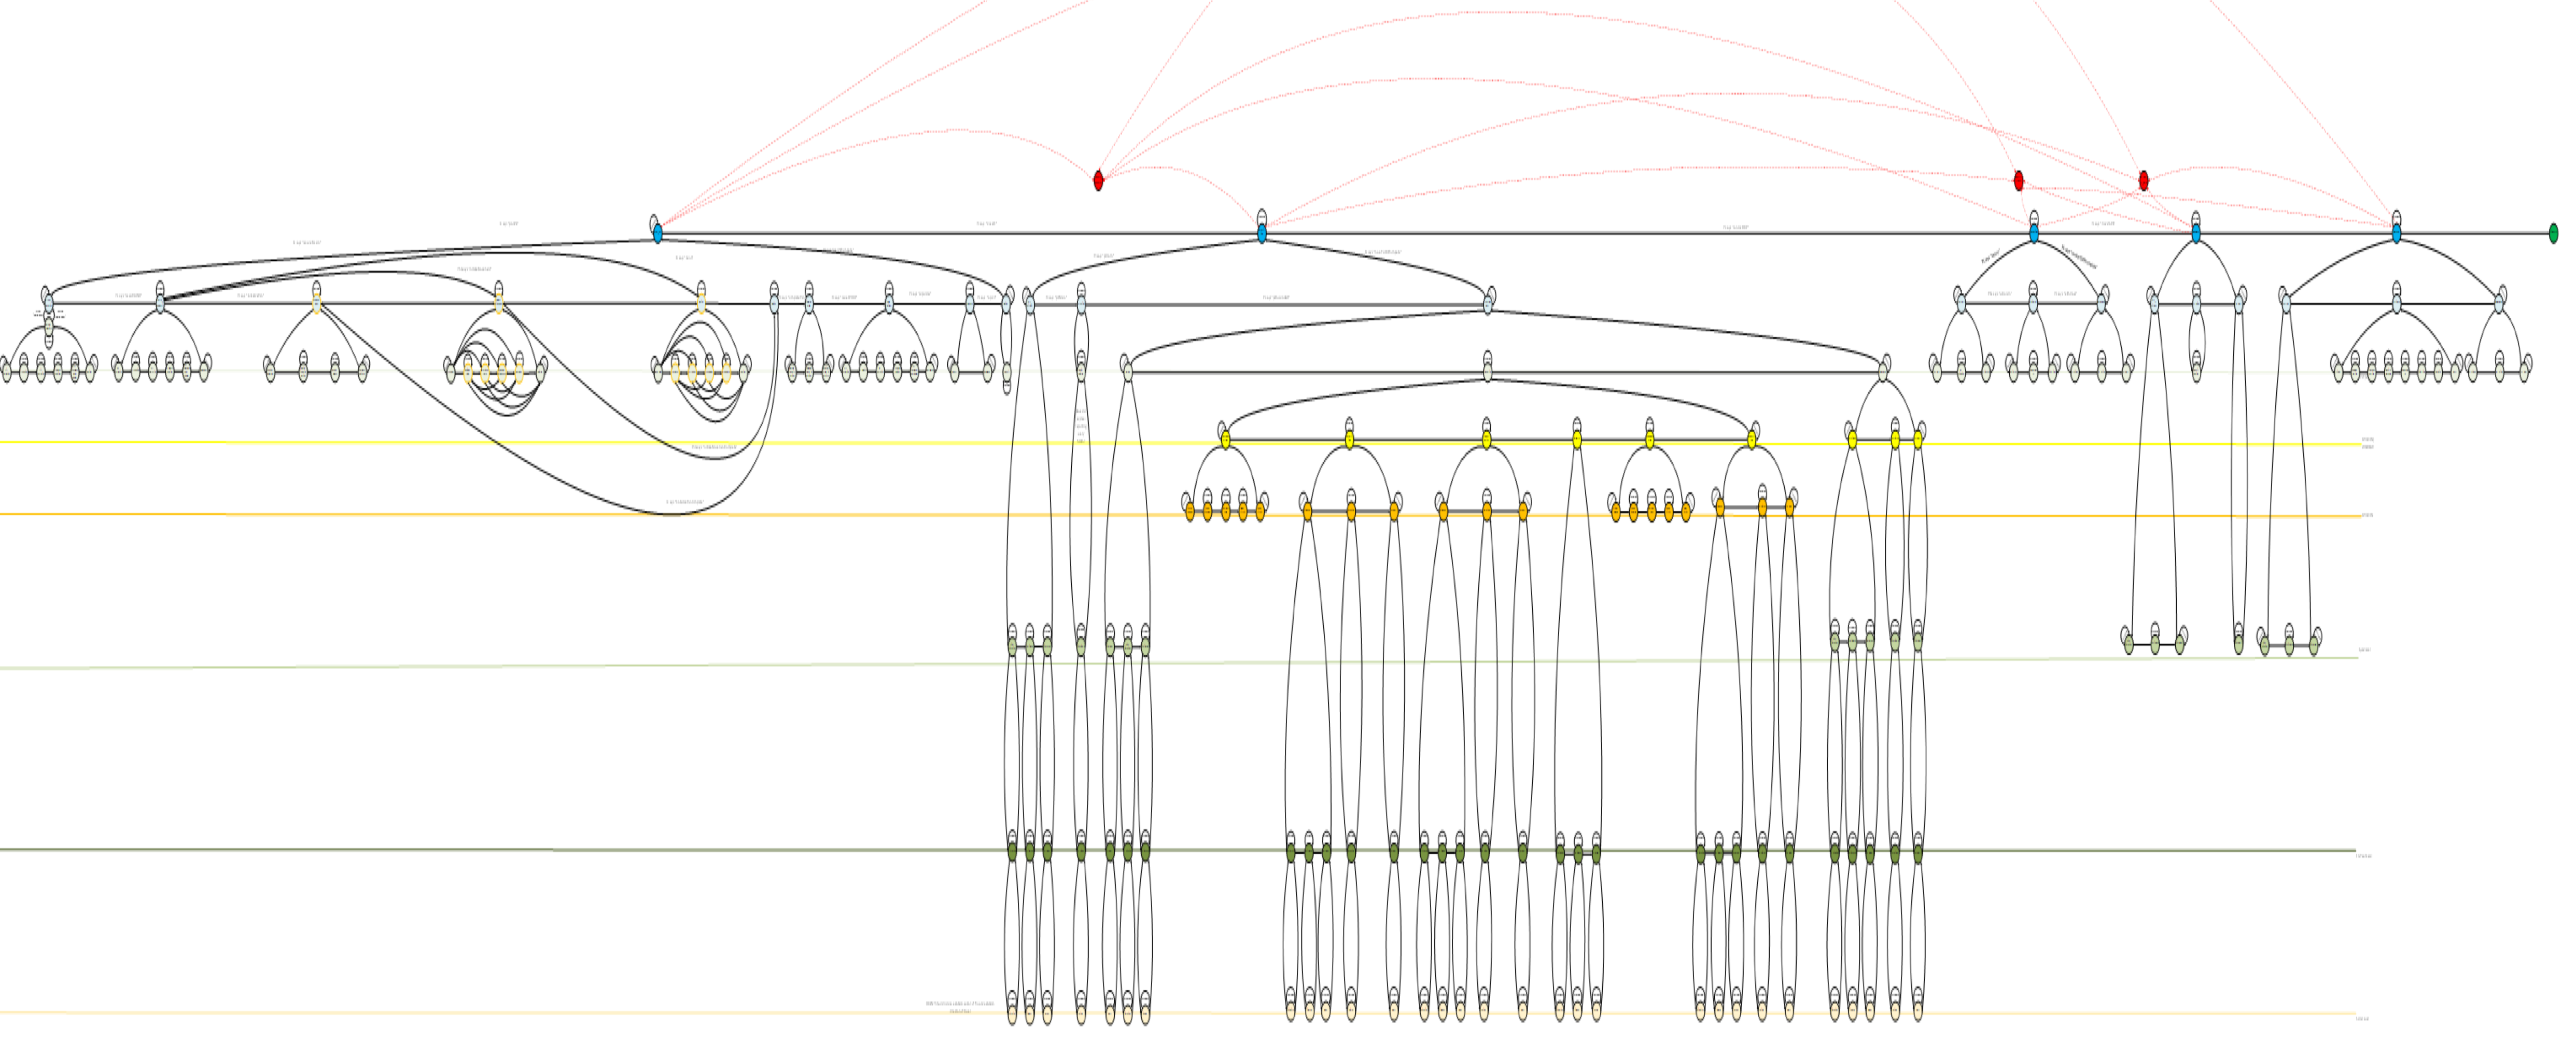
\includegraphics[width=\textwidth]{../figures/overalldiagramsquashed}
\caption{\label{overalldiagramsquashed}Diagrammatic description of patrol base operations as a modularized hierarchy of secure state machines.  (Generated by Jesse Nathaniel Hall.)}
\end{figure}

          %%%%%%%%%%%%%%%% Subsection Diagrammatic Description %%%%%%%%%%%%%%
\subsection{Diagrammatic Description in Visio}\label{ssec:overalldiagram}
The enormity of the hierarchy of \gls{ssm}s is evident in figure \ref{overalldiagramsquashed}.  This is a squashed version of the Visio diagram for the hierarchy of \gls{ssm}s. The diagram is included as a Visio file with the files for this project (LaTeX/figures/diagram.vis).  

\paragraph*{Levels of The Hierarchy}

The straight, colored lines that span the diagram in figure \ref{overalldiagramsquashed} delineate levels of the hierarchy of \gls{ssm}.  The top lines are obscured by the size of this squashed version of the diagram.  The most visible bright yellow line delineates the sub-sub-sub (4th) level of the hierarchy, for example.

Each level represents a different degree of abstraction with a set of principal responsible for actions at that level. 
\begin{itemize}
\item Red---escape level:\\
Unacceptable losses that require the mission to abort.  This is a floating module that can be reached by any level.
\item Dark blue--top level:\\
Describes the patrol base operations as five phases (plus an end phase).  The Platoon Leader (PL)  is responsible at this level.
\item Blue grey--sub-level:\\
This level takes the previous level's states to a lower level of abstraction.  The Platoon Leader and Platoon Sergeant (PSG) are responsible for this level.
\item Grey green--sub-sub-level:\\
This level takes the previous level's states to a lower level of abstraction.  The responsible principals are the patrol base headquarters: Platoon Leader, Platoon Sergeant, Radio Telephone Operator (RTO), Forward Observer (FO), Medic, and Heavy Weapons Squad Leader (HWSQL).
\item Bright yellow--4th level:\\
This level takes the previous level's states to a lower level of abstraction. The responsible principals are the squad leaders (SQL).
\item Orange--5th level:\\
This level takes the previous level's states to a lower level of abstraction.  The responsible principals are the Team Leaders (TL).
\item Olive--6th level:\\
This level takes the previous level's states to a lower level of abstraction.   The responsible principals are the Squads.  That is, the squad behavior is described at this level and the squad indicates readiness.
\item Dark green--7th level:\\
This level takes the previous level's states to a lower level of abstraction. The responsible principals are the Fire Team (FT), Recon Team (RT), Buddy Team (BT) and Security Team (ST).
\item Beige--8th level:\\
This level takes the previous level's states to a lower level of abstraction.  The responsible principals are the individual soldiers themselves.
\end{itemize}



The diagram is only a partial model of the patrol base operations.  The horizontal slice is the second to last row that expands across the diagram.  The vertical slice is in the middle of the diagram and expands several modules to the lowest level of abstraction.  

\paragraph*{States and Transitions in The Hiearchy}
The small, colored dots in figure \ref{overalldiagramsquashed} represent states (phases) of the patrol base operations.   The labels for these states are not readable in this diagram because of limited space, but each dot contains a description of the state.  The dots are color coded, with a different color for dots (states) at each level. 

The lines connecting one dot to another represent transition requests.  These lines are annotated, but are also unreadable in this diagram. 

The following sections describe modules from this diagram.  The descriptions of the states and transitions are discussed and a readable diagram for each model is provided.  


\subsection{Descriptions of Individual Modules}
Each module is described diagrammatically in the following sections.  They all follow a similar pattern.  The general pattern is discussed in this section.  Exceptions are discussed along with the diagrammatic descriptions for each individual module. (Note also that "module" and "SSM" are used interchangeably in the following sections.)

\paragraph*{Flow}
Each module follows a sequential pattern.\footnote{The patrol base operations are modeled as sequential activities.  However, not all operations follow a definite sequential pattern.  The planning phase discusses non-linear transitions.  Linear sequences are modeled because it is easier to work with given the complexity.  But, linear sequences are not necessary.}  It starts at one state and then flows sequentially to the end of the module. Each module has a set of principals who are authorized on some set of transitions (or commands).  Each module has its own security policy that dictates the conditions under which transition requests are granted.  

\paragraph*{Requests And Security Policies}
Principals make requests to transition from one state to another.  Requests are of the form \textit{Principal says command}.  

There are two approaches to the policy.  The first allows transition within each module with no regard to completion of lower level modules.  For example, transition from the planning phase to the move to \gls{orp} phase in the top level does not require any specific information about completion of the planning module in the level below.

The second approach requires confirmation of completion of the lower level module before transitions at the top level are allowed.  For example, before transitioning from the planning phase to the move to \gls{orp} phase, the planning phase must confirm that the planning module is complete.   This isn't necessarily true of the real patrol base operations.  For example, the patrol may move to the \gls{orp} before receiving it's mission.  But, modeling it this way demonstrates integration modules at different levels of the hierarchy. 

For this second approach, an "all knowing" principal (essentially a signal relay) communicates when a lower level module is complete.  This principal is called OMNI. OMNI allows for encapsulation of each module by communicating information about one module to another and eliminating the need for principals in one module to "know" what is happening in another module.  This is necessary to reason with the \gls{acl} in \gls{hol}.  It is a feature of the model and not the operations.


\paragraph*{Diagrammatic Description}
The colors of the states in the diagrams correspond to their colors in the overall squished diagram shown in figure \ref{overalldiagramsquashed}.  

All lines represent allowable transitions with an arrow indicating the direction of the transition.  Each line is annotated with the appropriate \gls{acl} request (or command).  The last line in each module is an exception.  It connects the COMPLETE state to the initial state.  This line is not annotated. In \gls{ssm}s that integrate modules, this could be thought of as feedback from OMNI.

\paragraph*{Naming conventions}
What follows are the naming conventions for the diagrams.  They also apply to the \gls{hol} implementation of the \gls{ssm}.
\begin{description}
\item[state: ] all capital letters with underscores representing spaces.  Examples include: MOVE_TO_ORP, PLAN_PB, etc.
\item[commands (or requests):] first letter is lower case.  The remaining letters toggle with a capital letter for each new word.  Examples include: moveToORP,  receiveMission, etc.  Furthermore, all commands take the name of the next state. For example, the transition from the state MOVE_TO_PB to CONDUCT_PB is conductPB.  The transition from the state COMPLETE_PLAN to ISSUE_OPORD is issueOPORD.  The only exception is the transition from the top level state PLAN_PB to the next state MOVE_TO_ORP.  The command for this transition is crossLD and not moveToORP.
\item[principals:] all begin with a capital letter then follow the convention for commands (or requests).  Examples include: PlatoonLeader, PlatoonSergeant, etc.
\item [\gls{acl} transition requests:] all are of the form \textit{Principal says command}.  Examples include: \textit{PlatoonLeader says moveToORP}, \textit{PlatoonSergeant says actionsIn}, etc.
\end{description}

          %%%%%%%%%%%%%%%% Subsection OMNI-Level %%%%%%%%%%%%%%%%%%%%%
\subsection{OMNI-Level}\label{ssec:omnilevel}
The OMNI level is not represented in the Visio diagram.  It is not really a level.  More specifically, the OMNI level represents an imaginary all-knowing entity.  The main purpose of this entity is to relay messages from one \gls{ssm} to another.  This allows for greater encapsulation of the modules. 

In all \gls{ssm}, OMNI is a principal who has authority over OMNI level commands.  These commands communicate the completion of a lower-level \gls{ssm}.  For example, at the top level, before the Platoon Leader can transition from the PLAN_PB state to the MOVE_TO_ORP state, he must receive the command \textit{OMNI says ssmPlanPBComplete}.  The top level security policy contains the clause \textit{OMNI controls ssmPlanPBComplete}.  The \textit{Controls} rule discussed in section \ref{ssec:inferencerules} then allows the Platoon Leader to conclude that the lower-level \gls{ssm} is complete.  
\clearpage

          %%%%%%%%%%%%%%%% Subsection Escape %%%%%%%%%%%%%%%%%%%%%%%
\subsection{Escape}\label{ssec:escape}
A diagram of the escape level is shown in figure \ref{escapeDiagram}.  The purpose of the escape level is to model situations wherein the patrol base operations must be aborted.  

\begin{figure}[h!]
\centering
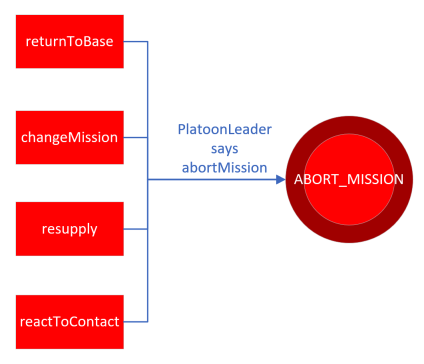
\includegraphics[width=0.45\textwidth]{../figures/escapeDiagram}
\caption{\label{escapeDiagram} Escape level diagram.}
\end{figure}

The square boxes in the diagram represent communication from outside the module.  They represent external signals from OMNI.  The only state is the ABORT_MISSION state. 

The abortable conditions are \textit{returnToBase}, \textit{changeMission}, \textit{resupply}, and \textit{reactToContact}.\footnote{React to contact in this description refers to unwanted contact that requires the mission to be aborted.  It does not refer to planned contact in combat missions or contact that does not require mission abortion.}


The security policy for the escape level contains the clauses \textit{OMNI controls returnToBase}, \textit{OMNI controls changeMission}, etc.  Given a request \textit{OMNI says returnToBase} and the security policy, \textit{returnToBase} is believed.  

The security policy also contains a clause that allows the Platoon Leader to transition to the ABORT_MISSION state if \textit{returnToBase} (\textit{changeMission}, etc.)  is believed and the Platoon Leader requests the transition.


 \clearpage

          %%%%%%%%%%%%%%%% Subsection Top Level %%%%%%%%%%%%%%%%%%%%%%
\subsection{Top Level}\label{ssec:toplevel}
The top level for the hierarchy is shown in figure \ref{ssmPBDiagram}.  This is a linearized version of figure \ref{pbtoplevel}.

\begin{figure}[h!]
\centering
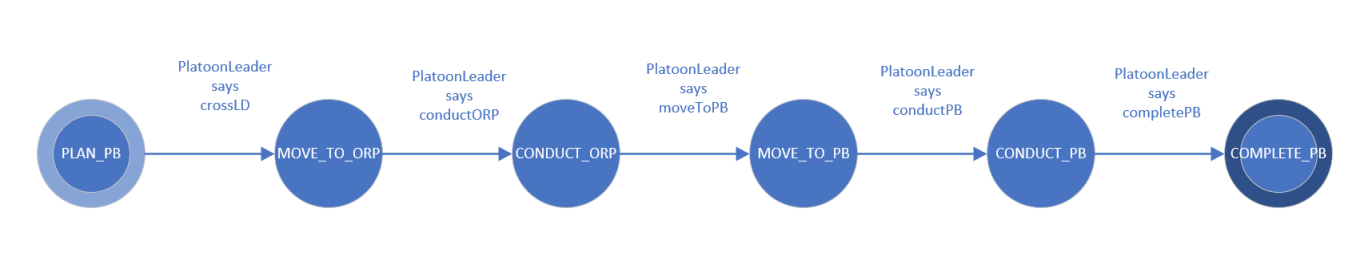
\includegraphics[width=\textwidth]{../figures/ssmPBDiagram}
\caption{\label{ssmPBDiagram} Top level diagram.}
\end{figure}

This \gls{ssm} represents the phases shown in figure \ref{pbtoplevel}.  There are six states: PLAN_PB, MOVE_TO_ORP, CONDUCT_ORP, MOVE_TO_PB, CONDUCT_PB, and COMPLETE_PB (an end state).  

Commands to transition from one state to another are named after the next state.  For example, to transition from MOVE_TO_ORP to CONDUCT_ORP, the command is conductORP.  The transition from the PLAN_PB state to the MOVE_TO_ORP state is the only exception.  This command is crossLD.  

Transitions are initiated by a request from and authenticated and authorized principal.  These requests have the form \textit{PlatoonLeader says crossLD}.

This \gls{ssm} integrates with the lower level modules.  This means that transitions are allowed when the appropriate lower level module is complete.  This requires the aid of the OMNI principal.

The Platoon Leader is the only authenticated principal at this level.  Authentication is assumed to be visual or other recognition (i.e., does not require anything complicated such as a cryptographic key.)

The security policy is state dependent.  It requires a signal from OMNI that the lower level module is complete.  Once this is believed, the Platoon Leader is authorized to make a transition to the next state.  

 \clearpage

          %%%%%%%%%%%%%%%% Subsection Horizontal Slice %%%%%%%%%%%%%%%%%%%
\subsection{Horizontal Slice}\label{ssec:horizontalslice}
The horizontal slice is an expansion of the states in the top level \gls{ssm}.  Each state (save for the COMPLETE_PB state) is expanded into an \gls{ssm}.  These \gls{ssm}s are described next.

                  %%%%%%%%%%%%% Subsection ssmPlanPB %%%%%%%%%%%%%%%%%%%%%
\subsubsection{ssmPlanPB}\label{sssec:ssmPlanPB}
The top level PLAN_PB state is expanded into the ssmPlanPB \gls{ssm} and shown in figure \ref{ssmPlanPBDiagram}.

\begin{figure}[h!]
\centering
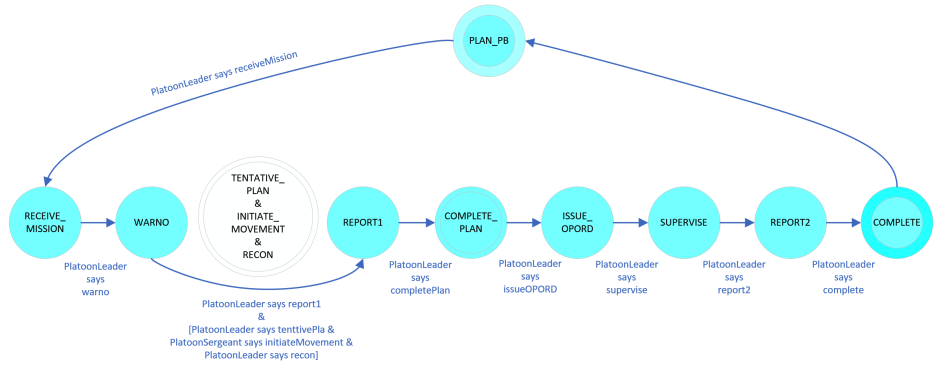
\includegraphics[width=\textwidth]{../figures/ssmPlanPBDiagram}
\caption{\label{ssmPlanPBDiagram} Horizontal slice: PlanPB diagram.}
\end{figure}

This is the largest \gls{ssm} and models the eight steps of the troop leading procedures.  

There are states: RECEIVE_MISSION, WARNO, TENTATIVE_PLAN, INITIATE_MOVEMENT, RECON, REPORT1, COMPLETE_PLAN, ISSUE_OPORD, SUPERVISE, REPORT2, and COMPLETE.

Transition commands follow the same pattern as in the other \gls{ssm}s.  The exception is discussed below.

All transitions are sequential.  However, the original module contains three non-sequential states.  These are represented in the diagram as the white circle. These states are TENTATIVE_PLAN, INITIATE_MOVEMENT, and RECON.  To transition from WARNO to REPORT1 requires that all three of these states be completed, but not in any specific order.
To solve this problem, the three states are not represented as states.  The completion of these "tasks" is indicated by the following three statements: \textit{PlatoonLeader says tentativePlan}, \textit{PlatoonSergeant says initiateMovement}, and \textit{PlatoonLeader says recon}.  Thus, the transition from WARNO to REPORT1 now requires four statements: \textit{PlatoonLeader says tentativePlan}, \textit{PlatoonSergeant says initiateMovement}, \textit{PlatoonLeader says recon}, \textbf{AND} \textit{PlatoonLeader says report1}. The latter-most statement is the actual request.  The security policy enforces this transition by including the clause \textit{tentativePlan andf initiateMovement andf recon impf PlatoonLeader controls report1}.  

ssmPlanPB has two principals: PlatoonLeader and PlatoonSergeant.  Only the PlatoonLeader is authorized to make transitions among states.  The PlatoonSergeant controls the InitiateMovement command (but, it is not a state and therefore there is no transition).

This \gls{ssm} does not integrate and thus does not require the OMNI principal.  The security policy authorizes the Platoon Leader to make transitions as described in previous sections, with the exception as described above.  


\clearpage
                  %%%%%%%%%%%%% Subsection ssmMoveToORP %%%%%%%%%%%%%%%%%%%
\subsubsection{ssmMoveToORP}\label{sssec:ssmMoveToORP}
The top level MOVE_TO_ORP state is expanded into the ssmMoveToORP \gls{ssm} and shown in figure \ref{ssmMoveToORPDiagram}.

\begin{figure}[!h]
\centering
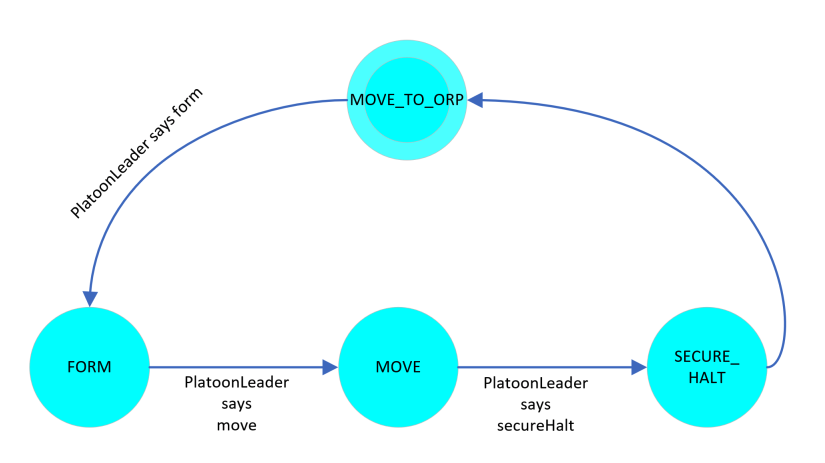
\includegraphics[width=0.8\textwidth]{../figures/ssmMoveToORPDiagram}
\caption{\label{ssmMoveToORPDiagram} Horizontal slice: MoveToORP diagram.}
\end{figure}

This \gls{ssm} has three states: FORM, MOVE, and SECURE_HALT.  

The Platoon Leader is the only authorized principal.  

This is an integrating \gls{ssm}, and requires a signal from OMNI that the lower level \gls{ssm} is complete.

The security policy allows for transitions if requested to do so from the Platoon Leader.  

\clearpage

                  %%%%%%%%%%%%% Subsection ssmConductORP %%%%%%%%%%%%%%%%%%
\subsubsection{ssmConductORP}\label{sssec:ssmConductORP}
The top level CONDUCT_ORP state is expanded into the ssmConductORP \gls{ssm} and shown in figure \ref{ssmConductORPDiagram}.


\begin{figure}[h!]
\centering
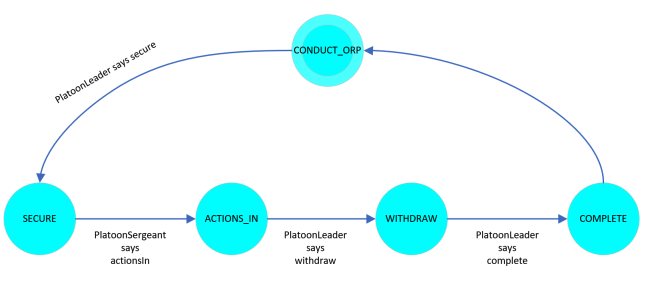
\includegraphics[width=\textwidth]{../figures/ssmConductORPDiagram}
\caption{\label{ssmConductORPDiagram} Horizontal slice: ConductORP diagram.}
\end{figure}


This \gls{ssm} has four states: SECURE, ACTIONS_IN, WITHDRAW, and COMPLETE.  

There are two principals.  The Platoon Leader is authorized on all commands except for the actionsIn command.  The PlatoonSergeant is only authorized on the actionsIn command.

In contrast to ssmMoveToORP, this is not an integrating \gls{ssm}, therefore there is no OMNI principal.  

The security policy allows for transitions if requested to do so from the Platoon Leader or the PlatoonSergeant.  

\clearpage

                  %%%%%%%%%%%%% Subsection ssmMoveToPB %%%%%%%%%%%%%%%%%%%
\subsubsection{ssmMoveToPB}\label{sssec:ssmMoveToPB}
The top level MOVE_TO_PB state is expanded into the ssmMoveToPB \gls{ssm} and shown in figure \ref{ssmMoveToPBDiagram}.

\begin{figure}[h!]
\centering
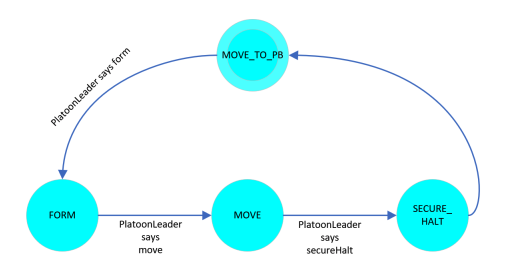
\includegraphics[width=0.8\textwidth]{../figures/ssmMoveToPBDiagram}
\caption{\label{ssmMoveToPBDiagram} Horizontal slice: MoveToPB diagram.}
\end{figure}

This \gls{ssm} is the same as ssmMoveToORP.  It has three states: FORM, MOVE, and SECURE_HALT.  

The Platoon Leader is the only authorized principal.  

In contrast to ssmMoveToORP, this is not an integrating \gls{ssm}, therefore there is no OMNI principal.  

The security policy allows for transitions if requested to do so from the Platoon Leader.  
\clearpage
                  %%%%%%%%%%%%% Subsection ssmConductPB %%%%%%%%%%%%%%%%%%%
\subsubsection{ssmConductPB}\label{sssec:ssmConductPB}
The top level CONDUCT_PB state is expanded into the ssmConductPB \gls{ssm} and shown in figure \ref{ssmConductPBDiagram}.

\begin{figure}[h!]
\centering
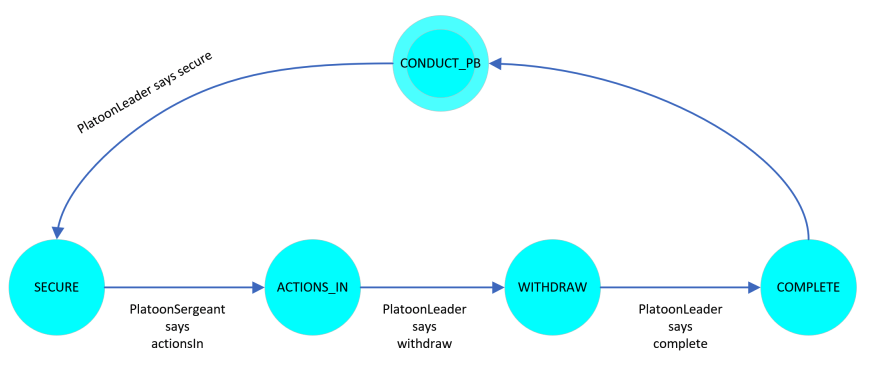
\includegraphics[width=\textwidth]{../figures/ssmConductPBDiagram}
\caption{\label{ssmConductPBDiagram} Horizontal slice: ConductPB diagram.}
\end{figure}

This \gls{ssm} is the same as ssmConductORP.  It has four states: SECURE, ACTIONS_IN, WITHDRAW, and COMPLETE.  

There are two principals.  The Platoon Leader is authorized on all commands except for the actionsIn command.  The PlatoonSergeant is only authorized on the actionsIn command.

In contrast to ssmMoveToORP, this is not an integrating \gls{ssm}, therefore there is no OMNI principal.  

The security policy allows for transitions if requested to do so from the Platoon Leader or the PlatoonSergeant.  


          %%%%%%%%%%%%%%%% Subsection Vertical Slice %%%%%%%%%%%%%%%%%%%%
\subsection{Vertical Slice}\label{ssec:verticalslice}
The vertical slice is an expansion of one state at each level of the hierarchy.  It is the middle section in the overall, squished diagram in figure \ref{overalldiagramsquashed}.  This is the only section of the patrol base operations that are modeled through to the lowest level of abstraction.

The vertical slice starts at the top level state MOVE_TO_ORP.  This state is expanded into the ssmMoveToORP \gls{ssm}. In this sub level, the state SECURE_HALT is expanded into the ssmSecureHalt \gls{ssm}.  In this sub-sub-level \gls{ssm}, the state ORP_RECON is expanded into the ssmORPRecon \gls{ssm}.  In this \gls{ssm}, the state MOVE_TO_ORP is expanded into the ssmMoveToORP4L \gls{ssm}.  In this \gls{ssm}, the state FORM_RT is expanded into the ssmFormRT \gls{ssm}.  

\clearpage
                  %%%%%%%%%%%%% Subsection ssmSecureHalt %%%%%%%%%%%%%%%%%%%
\subsubsection{ssmSecureHalt}\label{sssec:ssmSecureHalt}
The sub-sub-level SECURE_HALT state is expanded into the ssmSecureHalt \gls{ssm} and shown in figure \ref{ssmSecurtHaltDiagram}.

\begin{figure}[h!]
\centering
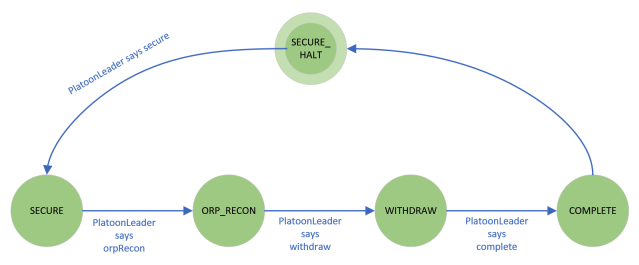
\includegraphics[width=0.85\textwidth]{../figures/ssmSecurtHaltDiagram}
\caption{\label{ssmSecurtHaltDiagram} Vertical slice: SecureHalt diagram.}
\end{figure}

This \gls{ssm} has four states: SECURE, ORP_RECON, WITHDRAW, and COMPLETE.  

The Platoon Leader is the only authorized principal.

This is not an integrating \gls{ssm}.  Therefore there is no OMNI principal.  

The security policy allows for transitions if requested to do so from the Platoon Leader.  

\clearpage

                  %%%%%%%%%%%%% Subsection ssmORPRecon %%%%%%%%%%%%%%%%%%%
\subsubsection{ssmORPRecon}\label{sssec:ssmORPRecon}
The sub-sub-sub-level ORP_RECON state is expanded into the ssmORPRecon \gls{ssm} and shown in figure \ref{ssmORPReconDiagram}.

\begin{figure}[h!]
\centering
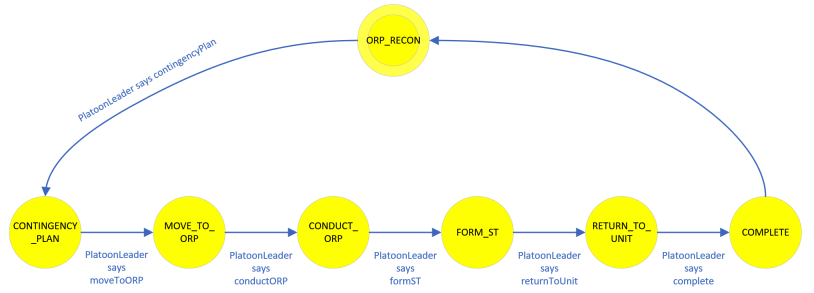
\includegraphics[width=\textwidth]{../figures/ssmORPReconDiagram}
\caption{\label{ssmORPReconDiagram} Vertical slice: ORPRecon diagram.}
\end{figure}

This \gls{ssm} has six states: CONTINGENCY_PLAN, MOVE_TO_ORP, CONDUCT_ORP, FORM_ST, RETURN_TO_UNIT, and COMPLETE.  

The Platoon Leader is the only authorized principal.

This is not an integrating \gls{ssm}.  Therefore there is no OMNI principal.  

The security policy allows for transitions if requested to do so from the Platoon Leader.  

\clearpage
                  %%%%%%%%%%%%% Subsection ssmMoveToORP4L %%%%%%%%%%%%%%%%%
\subsubsection{ssmMoveToORP4L}\label{sssec:ssmMoveToORP4L}
The 4th level MOVE_TO_ORP state is expanded into the ssmMoveToORP4L \gls{ssm} and shown in figure \ref{moveToORP4LDiagram}.  Recall that there is no module at the 5th level.  

\begin{figure}[h!]
\centering
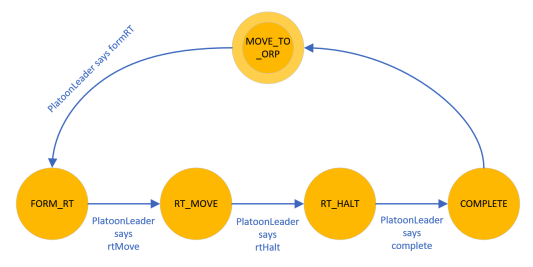
\includegraphics[width=0.85\textwidth]{../figures/moveToORP4LDiagram}
\caption{\label{moveToORP4LDiagram} Vertical slice: MoveToORP4L diagram.}
\end{figure}

This \gls{ssm} has four states: FORM_RT, RT_MOVE, RT_HALT, and COMPLETE.  

The Platoon Leader is the only authorized principal.

This is not an integrating \gls{ssm}.  Therefore there is no OMNI principal.  

The security policy allows for transitions if requested to do so from the Platoon Leader.

\clearpage

                  %%%%%%%%%%%%% Subsection ssmFormRT %%%%%%%%%%%%%%%%%%%%
\subsubsection{ssmFormRT}\label{sssec:ssmFormRT}
The 6th level FORM_RT state is expanded into the ssmFormRT \gls{ssm} and shown in figure \ref{moveToORP4LDiagram}.  (Note that there is no module at the 5th level for this slice.  Also, the 8th level is not modeled.)

\begin{figure}[h!]
\centering
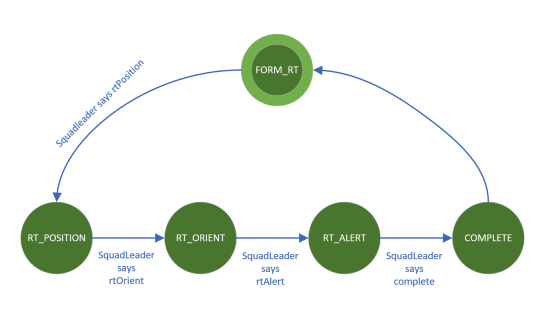
\includegraphics[width=0.85\textwidth]{../figures/ssmFormRTDiagram}
\caption{\label{ssmFormRTDiagram} Vertical slice: FormRT diagram.}
\end{figure}

This \gls{ssm} has four states: RT_POSITION, RT_ORIENT, RT_ALERT, and COMPLETE.  

The Platoon Leader is the only authorized principal.

This is not an integrating \gls{ssm}.  Therefore there is no OMNI principal.  

The security policy allows for transitions if requested to do so from the Platoon Leader.

The next chapter describes secure state machines in detail and discusses their implementation in \gls{hol}.
\end{document}